\documentclass[12pt]{article}
\usepackage{lingmacros}
\usepackage{tree-dvips}
\usepackage[T1]{fontenc}
\usepackage[polish]{babel}
\usepackage[utf8]{inputenc}
\usepackage{csquotes}
\usepackage{biblatex}
\usepackage{graphicx}
\usepackage{hyperref}
\usepackage{cleveref}
\bibliography{bibliography.bib}
\begin{document}
    \author{Juliusz Straszyński}
    \title{Raport końcowy projektu}
    \maketitle
    \tableofcontents


    \section{Wstęp}\label{sec:wstep}
    28 stycznia 2006 roku całą Polską wstrząsnęła tragedia — pod naporem śniegu zawaliła się hala MTK, w wyniku czego
    zginęło 65 osób.
    Po tym wydarzeniu firma WISENE Roof Monitoring opracowała rozwiązanie, które może zapobiec tego
    typu katastrofom.
    Projekt opiera się na zainstalowaniu szeregu precyzyjnych czujników mierzących odległość dachu
    od podłoża, dzięki czemu system może ostrzegać w sytuacji wykrycia nawet milimetrowych ugięć dachu.

    Siłą tego rozwiązania jest jego prostota — nie potrzeba skomplikowanego przygotowania, by zainstalować taki
    system.
    Dodatkowo są one tanie w utrzymaniu, zarówno materiałowo, jak i organizacyjnie.
    Są to niewątpliwe przewagi w stosunku do tensometrów.

    Natomiast wadą jest możliwe zaburzenie czujników.
    Przy zainstalowaniu takiego systemu w działających przedsiębiorstwach, nieuniknione jest potencjalne zastawianie
    czujnika.
    Zastawienia mogą być bardzo wyraźne -- np.\ po ustawieniu dwumetrowej szafy -- ale też mogą być
    delikatne — w wyniku pozostawienia paczki papierosów.

    Celem tego projektu było zażegnanie tego problemu poprzez opracowanie nowego, ulepszonego systemu raportującego,
    czy pomiar czujnika jest zastawiony, czy nie.
    Jest to istotny komponent systemu, bo jego brak może powodować zbyt
    częste raportowanie fikcyjnych ugięć, a to może prowadzić do ignorowania raportowanych alarmów.
    W miarę
    możliwości staramy się szacować faktyczne ugięcie, nawet gdy czujnik jest zastawiony.


    \section{Analiza danych}\label{sec:analiza-danych}

    \subsection{Struktura}\label{subsec:struktura}
    Otrzymaliśmy dostęp do 135 zestawów danych. Pojedynczy zestaw danych składa się z pomiarów z kilku czujników
    rozmieszczonych w różnych miejscach na pojedynczym obiekcie. Każdy czujnik charakteryzują następujące dane:
    \begin{itemize}
        \item identyfikator,
        \item baza pomiarów — jaką odległość od podłoża powinien domyślnie notować niezastawiony czujnik,
        \item seria pomiarów — notująca odległość czujnika od podłoża w kolejnych momentach.
    \end{itemize}
    Rozwiązanie zostało opracowane na podstawie pomiarów 1225 urządzeń i około 600 tys. pomiarów odległości.

    \subsection{Charakterystyka}\label{subsec:charakterystyka}

    \subsubsection{Odstępy czasu}
    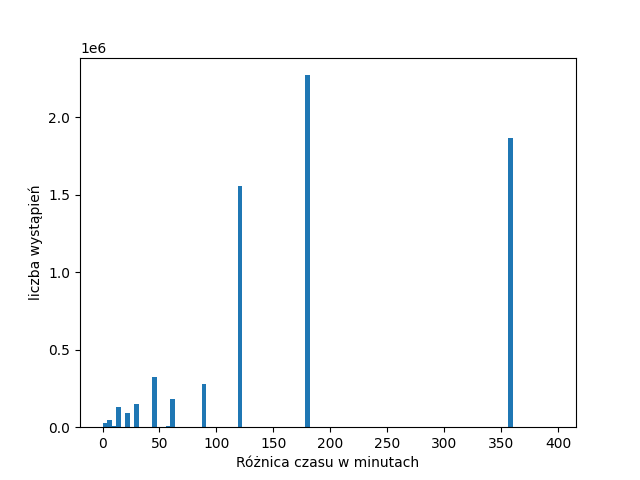
\includegraphics[width=\textwidth]{time_diff.png}
    Przez większość czasu pomiary są raportowane z częstotliwością 2, 3 lub 6 godzin. By ułatwić komputerową analizę,
    przepróbkujemy dane do mediany co 3h, wypełniając puste miejsca poprzednim notowaniem odległości, a zagęszczone
    przedziały normując do mediany. Mediana jest tutaj właściwym agregatorem, ponieważ jest ona odporna na duże
    odchylenia, w przeciwieństwie do np.\ średniej.

    \subsubsection{Różnice odległości}
    Przed przepróbkowaniem do 3 godzin mamy poniższy rozkład różnic odległości między kolejnymi pomiarami:

    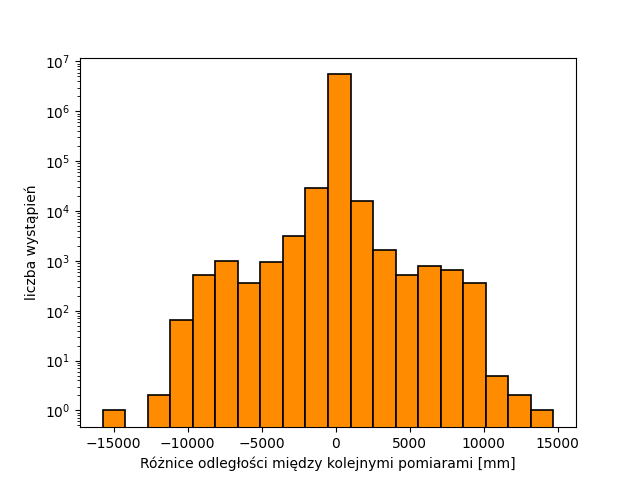
\includegraphics[width=\textwidth]{dist_diff_big.png}
    Bardzo istotne jest to, że pionowa skala jest logarytmiczna. Z informacji dostarczonych przez firmę wiadomo, że
    wychylenia w przeciągu kilku godzin mogą być co najwyżej 25-milimetrowe. Ta informacja pokrywa się z wyżej
    pokazanym wykresem. Bardzo wysoki szpic reprezentuje zdecydowaną większość obserwacji. Możemy również
    zaobserwować strzeliste rozkłady normalne dużych zastawień po bokach -- prawdopodobnie wysokich szaf, półek, itp.

    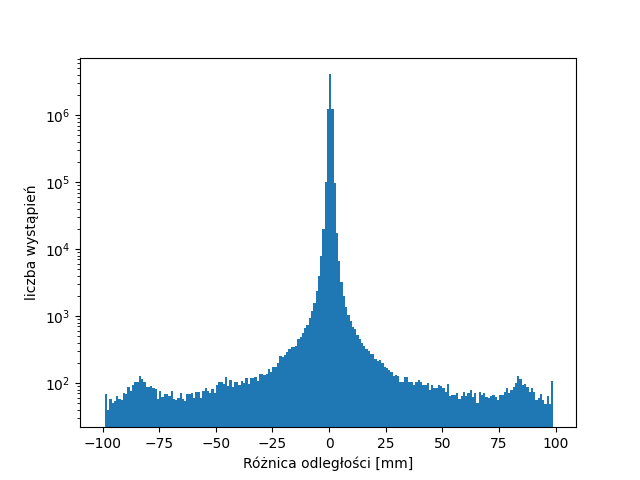
\includegraphics[width=\textwidth]{dist_diff_small.png}

    Po przepróbkowaniu rozkład pozostał bez większych zmian:

    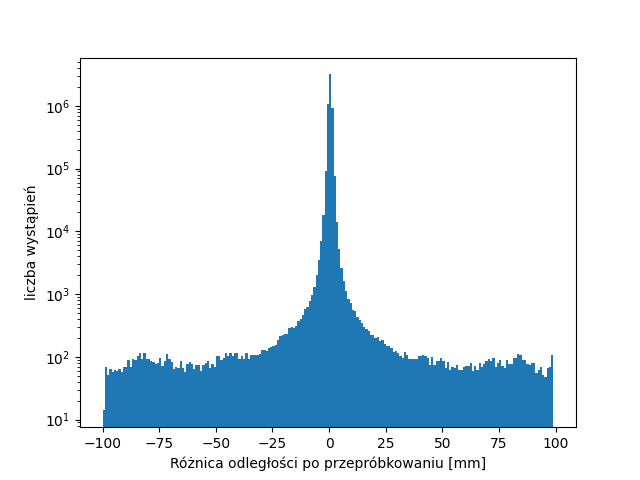
\includegraphics[width=\textwidth]{dist_diff_small_resampled.png}

    \subsubsection{Różnice bazy od odległości}

    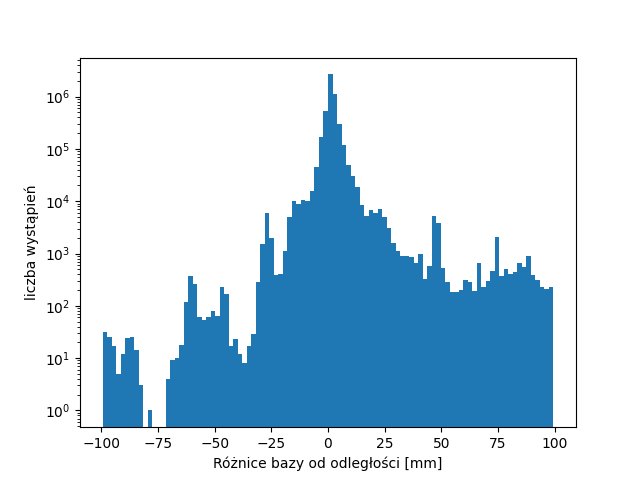
\includegraphics[width=\textwidth]{dist.png}

    Różnice poniżej zera są wynikiem źle skonfigurowanej bazy. Dane są ponownie przedstawione w skali logarytmicznej,
    bo w przeciwnym wypadku nie dałoby się niczego zauważyć. Zdecydowana większość obserwacji oscyluje wokół zera.
    Mediana jest równa zero. Będzie to kluczowe -- prawdziwe odkształcenia dachu powinny być krótkotrwałe i w
    dłuższej perspektywie mediana pomiarów powinna wynosić zero.

    \subsubsection{Przykłady danych}

    \subsubsection{Podsumowanie}


    \section{Metodologia i algorytm}\label{sec:metodologia-i-algorytm}

    \subsection{Wstęp}\label{subsec:wstep}
    Każdy zestaw danych składa się z kilku szeregów czasowych. W tych szeregach czasowych mamy zidentyfikować
    anomalie (ang.\ \emph{outlier}, \emph{anomaly}). Jest to znany problem w analizie statystycznej, do którego mamy
    do dyspozycji opracowane wcześniej narzędzia. Dziedziną zajmującą się rozpoznawaniem anomalii jest
    \emph{intervention analysis}.

    Prawdopodobnie najważniejszą pracą w tej dziedzinie jest praca Ruey S. Tsaya\citetitle{https://doi.org/10.1002/for.3980070102}\cite{https://doi.org/10.1002/for.3980070102}.
    Jest ona powszechnie cytowanym fundamentem współczesnej analizy anomalii w szeregach czasowych.

    Najistotniejsze jest zidentyfikować, czym tak naprawdę jest zastawienie z punktu widzenia intervention analysis.
    Zastawienie tymczasowo zmienia bazę pomiarów miernika. Oznacza to, że na czas zastawienia, pomiary są zmienione o
    pewną wysokość. Używając terminologii z ww. pracy jest to klasyfikowane jako \emph{level shift}. Jeśli
    zastawienie jest krótkotrwałe, to bardziej pasuje termin \emph{spike}.

    Praca Tsaya opiera się głównie na modelach \emph{ARMA}. Model ARMA jest połączeniem dwóch modeli AR i MA, czyli
    autoregresji i średniej kroczącej. Model (a konkretnie część MA) można stosować pod warunkiem, że analizowany
    szereg czasowy jest stacjonarny.

    Dodatkowo, by nasze rozwiązanie było możliwe do zastosowania w praktyce, musimy raportować wyniki na bieżąco, tj
    .\ w trybie \textbf{online}. Jest to kluczowe, ponieważ zmniejszy to użyteczność niektórych potencjalnych modeli.

    \subsection{Skorelowanie urządzeń}
    Jako że na urządzenia z pojedynczego budynku oddziałują praktycznie te same warunki atmosferyczne, to można by,
    zamiast modelu rozpatrującego każde z urządzeń osobno, spróbować wywnioskować anomalie z braku synchronizacji ruchów
    między urządzeniami.

    Nie zdecydowaliśmy się na to, ze względu na dwa czynniki. Po pierwsze model mógłby się przeuczyć (ang.\
    \emph{overfit}) na podstawie tej własności, co sprawiłoby, że fałszywie raportowałby zastawienie w przypadku, gdy
    tylko część dachu jest obciążona np.\ materiałami budowlanymi, zamiast śniegiem. Po drugie trenowanie modelu na
    wielowymiarowym szeregu czasowym jest dużo trudniejsze i łatwiej o przeuczenie się. Dlatego właśnie w praktyce, w
    takich sytuacjach, rozpatruje się szeregi czasowo niezależnie, o ile jest taka możliwość.

    \subsection{Metoda rozstępu ćwiartkowego}
    Metoda rozstępu ćwiartkowego (ang.\ IQR -- Interquartile range) jest jedną z najprostszych metod rozpoznawania
    anomalii w szeregu czasowym. Po poszeregowaniu historycznych danych na kwartyle $Q_1, Q_2, Q_3, Q_4$, definiujemy
    $\mathit{IQR}:= Q_3 - Q_1$, nazywane także \emph{midspread}. Następnie jesteśmy w stanie wykonać prosty
    Interquartile
    range test -- sprawdzamy, czy analizowany pomiar jest pomiędzy $Q_1 - c \cdot \mathit{IQR}$ i $Q_3 + c \cdot
    \mathit{IQR}$, gdzie $c$ to dopuszczalny margines. W naszym przypadku przyjęliśmy $c=3$, by tolerować szeroki zakres
    obserwacji.

    \subsection{Zmiana poziomu}\label[]{levelshift}
    Zmiana poziomu (ang.\ \emph{level shift}) jest jednym z głównych typów anomalii analizowanych w pracy
    \cite{https://doi.org/10.1002/for.3980070102}.
    By wykrywać takie anomalie, używa się podwójnego przesuwnego okna.
    Podwójne przesuwne okno jest parametryzowane przez $d$, oznaczające długość skrzydła.
    Jeśli ostatnie $2d$ pomiarów to $X_1, \ldots X_{2d}$, to lewym skrzydłem jest $X_1, \ldots X_d$, a prawym $X_{d +
    1}, \ldots, X_{2d}$. Metryką dla
    takiego podwójnego przesuwnego okna jest różnica median prawego i lewego skrzydła. Następnie dla tej metryki używamy
    metody rozstępu ćwiartkowego.

    Niestety nie jest to wskaźnik, którego moglibyśmy łatwo użyć w naszym przypadku. Daje on informację z opóźnieniem
    $d$
    obserwacji, ponieważ daje on informację o środkowym elemencie między skrzydłami. Dodatkowo, informacja ta jest
    zduplikowana -- po niewielkim przesunięciu okna ta metoda nadal notuje anomalię. Przez to ciężko odzyskać faktyczny
    poziom ugięcia dachu.

    \subsection{Nagłe wzrosty}\label{spike}
    Nagły wzrost (ang.\ \emph{spike}) jest kolejnym typem anomalii rozpatrywanym w pracy \cite{https://doi.org/10
    .1002/for.3980070102}. Ten typ anomalii jest wykrywany poprzez przesuwne okno, które jest parametryzowane przez $d$
    -- jego rozmiar. Jeśli ostatnie $d + 1$ pomiarów to $X_1, \ldots X_{d + 1}$, to oknem jest $X_1, \ldots X_d$.
    Metryką
    jest różnica ostatniego elementu $X_{d+1}$ od mediany okna. Dla takiej metryki używamy metody rozstępu ćwiartkowego.
    Metoda ta jest wykryje zmianę poziomu w najwcześniejszym momencie, ponieważ początek level shift jest również
    spikem.

    \subsection{Autoregresja}\label{autoregression}
    Autoregresja pozwala sprawdzić, czy obserwacje nie odbiegają od poprzedzających w ramach pewnej funkcji liniowej.
    Jest parametryzowana przez $d$ -- rozmiar okna. Jeśli ostatnie $d + 1$ pomiarów to $X_1, \ldots X_{d + 1}$, to oknem
    jest $X_1, \ldots X_d$. Dodatkowo, uczymy się parametrów $c_1, \ldots, c_d$. Metryką jest różnica ostatniego
    elementu
    $X_{d+1}$ od kombinacji liniowej $c_1X_1 + c_2X_2 + \ldots + c_dX_d$. Parametrów uczymy się za pomocą regresji
    liniowej na historycznych danych. Dla metryki używamy metody rozstępu ćwiartkowego. Jest to bardzo precyzyjna
    metoda,
    która dobrze działa, jeśli mamy wysoki poziom autokorelacji w szeregu czasowym. W naszym przypadku ten warunek jest
    spełniony.

    \subsection{Próg}\label{threshold}
    Znając możliwy potencjalny zakres danych, możemy pozbyć się z danych wejściowe najbardziej oczywistych anomalii,
    które mogłyby zaburzyć bardziej skomplikowane metody jak autoregresja. Każde urządzenie ma maksymalne możliwe
    ugięcie, po przekroczeniu którego powinien uruchomić się alarm. Możemy ustawić próg na najbardziej oczywiste
    anomalie
    na 4-krotność maksymalnego możliwego ugięcia, bo wtedy albo mamy zastawienie, albo dach powinien już się dawno
    zawalić.

    \subsection{Inżynieria danych}
    Nasze 135 zestawów danych zostało podzielone na dwie części -- testową i ewaluacyjną. Testowa część składa się z
    danych z 50 losowych urządzeń, natomiast pozostałe zostały wykorzystane do ewaluacji. Dane zostały przepróbkowane do
    okresu 3 godzin.

    \subsection{Rozwiązanie}\label{solution}
    Używamy wskaźników z sekcji \ref{spike}, \ref{autoregression} i \ref{threshold}, i obserwacja jest raportowana jako
    anomalia, jeśli dowolny z tych wskaźników zwróci, że obserwacja jest anomalią.

    \subsection{Odrzucone rozwiązania}
    Zamiast klasycznej analizy statystycznej, moglibyśmy również spróbować znanych metod uczenia maszynowego,
    przykładowo
    sieci neuronowych. Jednakże metody te najczęściej nie radzą sobie z danymi o wysokim poziomie szumu, a z takimi mamy
    do czynienia w naszym przypadku. Dodatkowo, nie ma problemu z trudnością z interpretowalnością wyników. Zagraniczne
    korporacje takie jak Facebook nadal używają klasycznych metod statystycznych do wykrywania anomalii \cite{Prophet},
    chociaż pojawiają się próby zaadaptowania do współczesnych metod uczenia maszynowego \cite{Neuralprophet}.

    Istniejące, bardziej skomplikowane rozwiązania takie jak Prophet Facebooka \cite{Prophet} skupiają się głównie na
    wahaniach sezonowych, ponieważ są one przeznaczone dla systemów o dużej skali, działających w czasie rzeczywistym. W
    naszym przypadku wahania sezonowe mają znaczenie drugorzędne - mimo że zwykle możemy spodziewać się opadów śniegu w
    zimie, to nie możemy na tym polegać, gdyż nadmierne obciążenia mogą powstać z innej przyczyny i nadal być
    niebezpieczne.


    \section{Realizacja}

    \subsection{Implementacja}
    Eksploracja danych i trenowanie zostały wykonane w języku programowania Python przy użyciu biblioteki ADTK
    \cite{ADTK} wydanej w 2019 roku. Następnie, po wytrenowaniu parametrów, program został przepisany na język C++ do
    postaci prostej biblioteki implementującej wskaźniki wymienione w sekcji \ref{solution}.
    \printbibliography
\end{document}
